\documentclass[unicode, notheorems]{beamer}
\usepackage{graphicx}
% If you have more than three sections or more than three subsections in at least one section,
% you might want to use the [compress] switch. In this case, only the current (sub-) section
% is displayed in the header and not the full overview.
\mode<presentation>
{
  \usetheme[numbers, totalnumbers, minimal]{Statmod}

\setbeamercovered{transparent}
  % or whatever (possibly just delete it)
{\tiny }}
\setbeamercolor{alerted text}{fg=blue}

%\usepackage{pscyr}
\usepackage[T2A]{fontenc}
\usepackage[utf8]{inputenc}
\usepackage[russian]{babel}
\usepackage{amsthm}

%\usepackage{tikz}
% you only need this when using TikZ graphics

\newtheorem{theorem}{Óòâåðæäåíèå}
\newtheorem{example}{Ïðèìåð}
\newtheorem{definition}{Îïðåäåëåíèå}
\newtheorem{task}{Çàäà÷à}
\newtheorem{def1}{Îïðåäåëåíèå}
\newtheorem{proposition}{Óòâåðæäåíèå}
\newtheorem{notice}{Çàìå÷àíèå}
\newtheorem{task_regul}{Çàäà÷à ñ ðåãóëÿðèçàöèåé}
\DeclareMathOperator{\sign}{sign}
\DeclareMathOperator*{\argmax}{arg\,max} 

\title[Нейронные сети для изображений]{Нейронные сети для изображений}

\author[Лунев И., Петраков М.]{Лунев Иван, \\ Петраков Михаил}
%\institute[ÑÏáÃÓ]{Ñàíêò-Ïåòåðáóðãñêèé ãîñóäàðñòâåííûé óíèâåðñèòåò \\
%    Ìàòåìàòèêî-ìåõàíè÷åñêèé ôàêóëüòåò \\
%    Êàôåäðà ñòàòèñòè÷åñêîãî ìîäåëèðîâàíèÿ \\
%    \vspace{0.4cm}
%    Íàó÷íûé ðóêîâîäèòåëü: ê.ô.-ì.í., äîö. Ãîëÿíäèíà Í.Ý. \\
%    Ðåöåíçåíò: ì.í.ñ. Øëåìîâ À.Þ.
%        \vspace{0.3cm}
%}
\date{
    Санкт-Петербург\\
    2019г.
}

\subject{Beamer}
% This is only inserted into the PDF information catalog. Can be left
% out.

% Delete this, if you do not want the table of contents to pop up at
% the beginning of each subsection:
% \AtBeginSubsection[]
% {
%   \begin{frame}<beamer>
%     \frametitle{Outline}
%     \tableofcontents[currentsection,currentsubsection]
%   \end{frame}
% }

\begin{document}

\begin{frame}
    \titlepage
\end{frame}


% \begin{frame}
%     \frametitle{Классификация изображений}
%  \begin{figure}[h]
% 	\begin{center}
% 		\begin{minipage}[h]{1\linewidth}
% 			\includegraphics[width=1\linewidth]{1}
% 		\end{minipage}
% 	\end{center}
% \end{figure}
 
%\end{frame}

\begin{frame}
\frametitle{Структура CNN}

%\alert{Ìåòîä:} ìåòîä ñòîõàñòè÷åñêîãî ãðàäèåíòà.
Сверточная нейронная сеть состоит из разных видов слоев:

\begin{itemize}
	\item сверточные (convolutional) слои
	\item объединяющие слои (pooling layer)
	\item полносвязные слои
\end{itemize}
\begin{figure}[h]
	\begin{center}
		\begin{minipage}[h]{0.70\linewidth}
			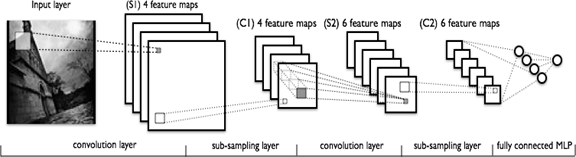
\includegraphics[width=1\linewidth]{structure}
		\end{minipage}
	\end{center}
\end{figure}

% \begin{figure}[h]
% 	\begin{center}
% 		\begin{minipage}[h]{0.70\linewidth}
% 			\includegraphics[width=1\linewidth]{mn}
% 		\end{minipage}
% 	\end{center}
% \end{figure}
\end{frame}

\begin{frame}
	\frametitle{Количество параметров}
	В снс количество параметров сокращается.\\
	Рассчитаем кол-во параметров для нс:
		$n = (i * h + h * o) + (h + o)$, где $i$ -- размер входного слоя, $h$ -- размер скрытого слоя, $o$ -- размер выходного слоя $n = (3 * 5 + 5 * 2) + (5 + 2) = 32$
	\begin{figure}[h]
	\begin{center}
		\begin{minipage}[h]{0.4\linewidth}
			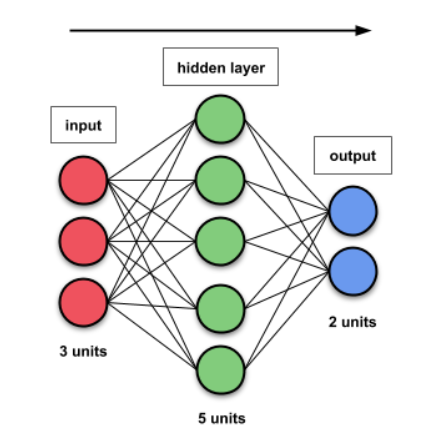
\includegraphics[width=1\linewidth]{ex1}
			\end{minipage}
			\begin{minipage}[h]{0.4\linewidth}
			\includegraphics[width=1\linewidth]{ex2}
		\end{minipage}
	\end{center}
	Рассчитаем кол-во параметров для снс:
	$n = [ x * ( w * w ) * o ] + o = [3 * (2 * 2) * 1] + 1 = 13$
\end{figure}



% 	\begin{figure}[h]
% 	\begin{center}
% 		\begin{minipage}[h]{0.30\linewidth}
% 			\includegraphics[width=1\linewidth]{ex2}
% 		\end{minipage}
% 	\end{center}
% \end{figure}


\end{frame}

\begin{frame}
	\frametitle{Сверточный слой}
	
	$\mathsf{x}[i,j]$ - исходные признаки, пиксели $n \times m$ изображения; \\
	$\mathsf{w}_{ab}$ - ядро свертки, где считаем, что ядро является прямоугольным, а a и b длины его сторон;%, $\mathsf{a} = -A,\dots,+A$, $\mathsf{b} = -B,\dots,+B$
	 \\
	Сверточный нейрон: %с (2A+1)(2B+1) весами:
	\begin{center}
		% $(\mathsf{x} * \mathsf{w})[\mathsf{i},\mathsf{j}] = \sum \limits_{\mathsf{a} = -A}^{A} \sum \limits_{\mathsf{b} = B}^{B} \mathsf{w}_{\mathsf{ab}} \mathsf{x}[\mathsf{i} + \mathsf{a}, \mathsf{j} + \mathsf{b}]$
		$(\mathsf{x} * \mathsf{w})[\mathsf{i},\mathsf{j}] = \sum \limits_{\mathsf{a}} \sum \limits_{\mathsf{b}} \mathsf{w}_{\mathsf{ab}} \mathsf{x}[\mathsf{i} + \mathsf{a}, \mathsf{j} + \mathsf{b}]$
	\end{center}
	%  $\mathsf{x}[i,j]$ - исходные признаки, пиксели $n \times m$ изображения \\
	%  $\mathsf{w}$ - ядро свертки \\
	%  Сверточный нейрон с весами:
	%  \begin{center}
	%  	$(\mathsf{x} * \mathsf{w})[\mathsf{i},\mathsf{j}] = \sum_{k,l} \mathsf{x}[\mathsf{i} - k, \mathsf{j} - l] * w[k,l] $
	% \end{center}

	% \begin{center}
	% \begin{equation*}
	% 	$(I \times K)_{ij} = \sum \limits_{m=0}^{k_{1}-1} \sum \limits_{n=0}^{k_{2}-1} I(i-m,j-n)K(m,n) = \sum \limits_{m=0}^{k_{1}-1} \sum \limits_{n=0}^{k_{2}-1} I(i+m,j+n)K(-m,-n)$
	% \end{equation*}
	% \end{center}
	

\begin{figure}[h]
	\begin{center}
		\begin{minipage}[h]{0.72\linewidth}
			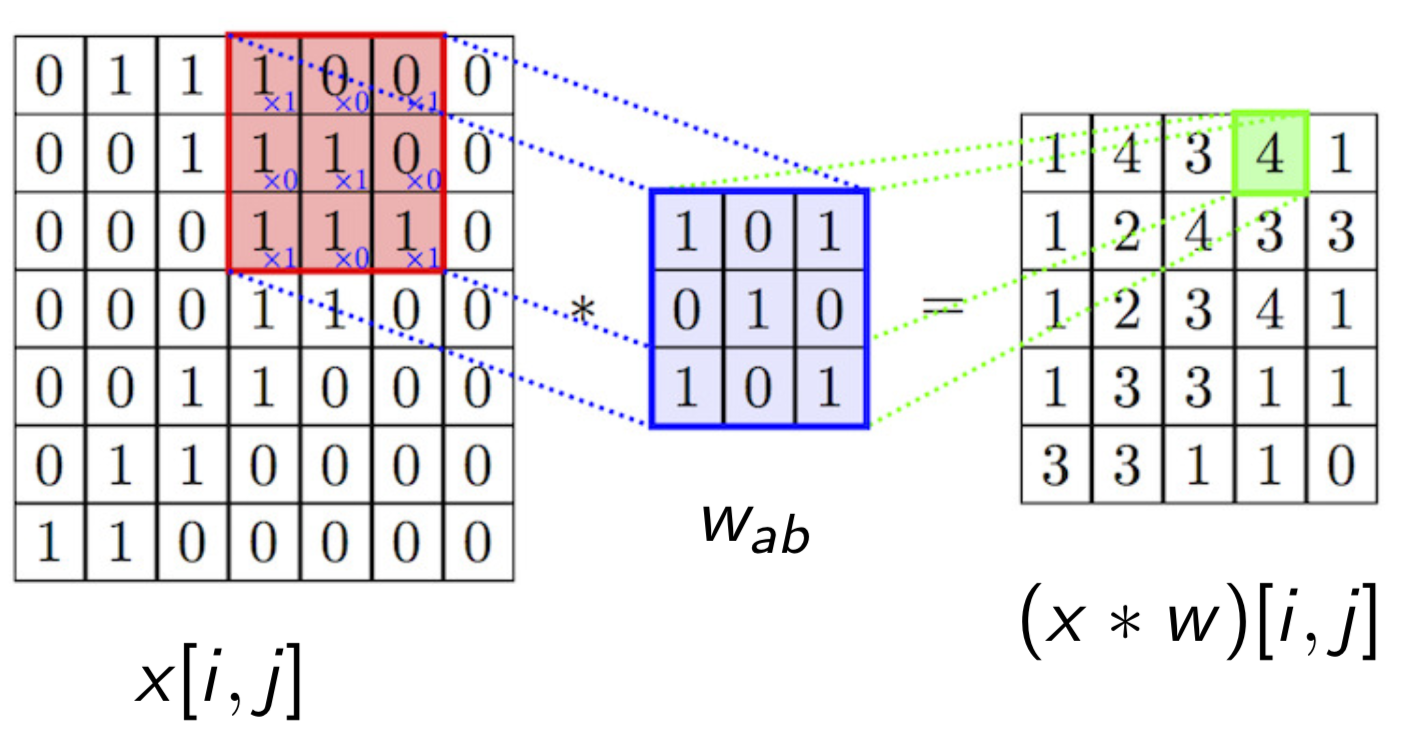
\includegraphics[width=1\linewidth]{sv}
		\end{minipage}
	\end{center}
\end{figure}

\end{frame}

\begin{frame}
	\frametitle{Сверточный слой (Пример)}
	Например, пусть вход имеет размер $[32 \times 32 \times 3]$. В этом случае возьмем размер фильтра  $[5 \times 5 \times 3]$, то есть фильтр будет иметь форму прямоугольного параллелепипеда, в общей сложности $5 * 5 * 3 = 75$ весовых коэффициентов (и $+1$ параметр смещения). Используются параллельно несколько разных фильтров, за счет чего сеть растет "вглубь".
		\begin{figure}[h]
			\begin{center}
				\begin{minipage}[h]{0.9\linewidth}
					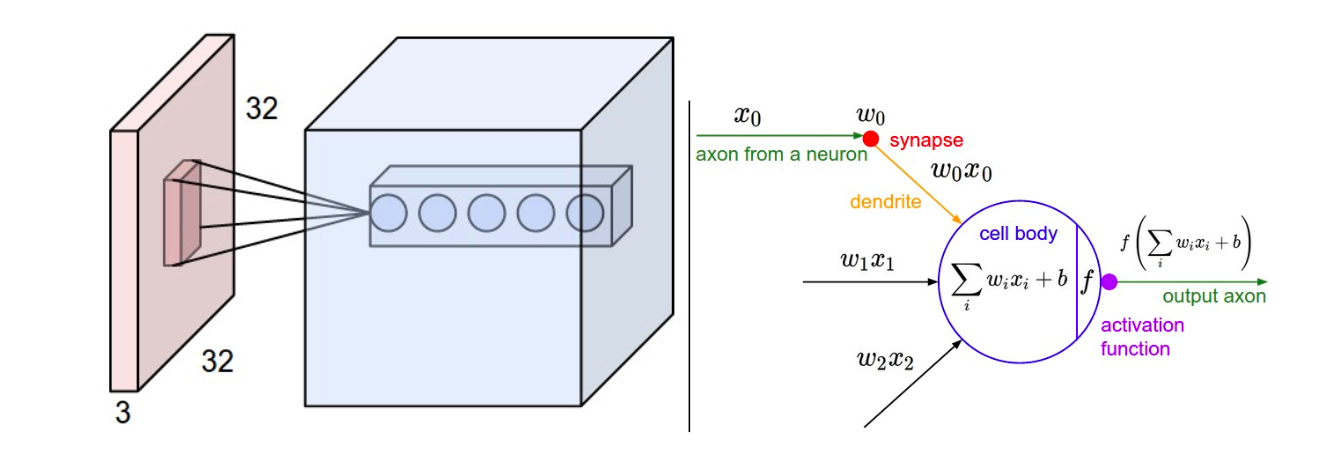
\includegraphics[width=1\linewidth]{sv1}
				\end{minipage}
			\end{center}
		\end{figure}

\end{frame}

\begin{frame}
	\frametitle{Сверточный слой (Пример)}
	Гиперпараметры, формирующие размер выхода сверточного слоя:
	 \begin{itemize}
	 	\item глубина (depth) --- количество разных фильтров
	 	\item шаг (stride) --- шаг сдвига фильтра
	 	\item дополнение нулями (zero-padding)
	 \end{itemize}

	 Для одномерного случая: $(W-F+2P)/S+1$ - размер выходного слоя, где $W$ - размер входа, $F$ - ширина фильтра, $P$ --- заполнение $0$, $S$ --- шаг.

	 $F = 3$, $W = 5$, $P = 1$.
	 \begin{itemize}
	 	\item[left] - $S = 1$, следовательно размер выхода $(5 - 3 + 2) / 1 + 1 = 5$
	 	\item[right] - $S = 2$, следовательно размер выхода $(5 - 3 + 2) / 2 + 1 = 3$
	 \end{itemize}
	 \begin{figure}[h]
			\begin{center}
				\begin{minipage}[h]{0.9\linewidth}
					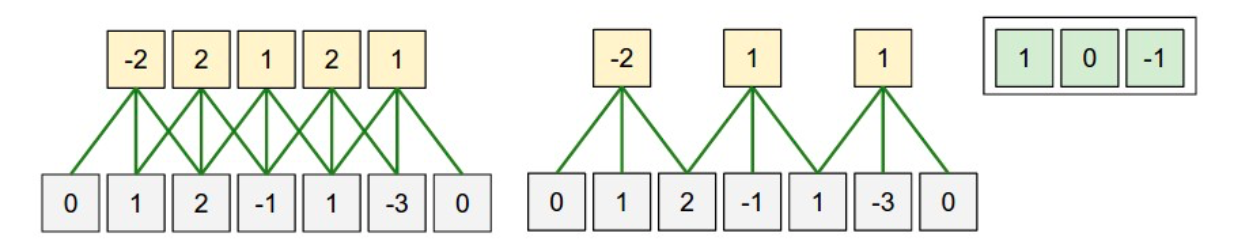
\includegraphics[width=1\linewidth]{sv2}
				\end{minipage}
			\end{center}
		\end{figure}
\end{frame}

\begin{frame}
	\frametitle{Сверточный слой (Итоги)}
	\begin{center}
		\begin{itemize}
			\item вход размером $W_{1} \times H_{1} \times D_{1}$ (обычно рассматриваются картинки, у которых глубина (RGB) равна $D_{1}=3$)
			\item требует 4 гиперпараметра :
				\begin{itemize}
			 		\item $K$ -- количество фильтров
			 		\item $F$ -- размер фильтра (имеется ввиду трехмерный квадратный фильтр со стороной F и глубиной $D_{1}=3$, но вообще говоря форма может быть любой)
			 		\item $S$ -- шаг свертки
			 		\item $P$ -- заполнение нулями (ширина полосы по кругу картинки, которые заполняются нулями)
				\end{itemize}
			\item на выходе $W_{2} \times H_{2} \times D_{2}$
				\begin{itemize}
					\item $W_{2}  = (W_{1} - F + 2P)/S + 1$
					\item $H_{2}  = (H_{1} - F + 2P)/S + 1$
					\item  $D_{2} = K$
				\end{itemize}
			\item $F*F*D_{1}$ весов на фильтр, всего $F*F*D_{1}*K$ весов
			\item Далее к получившимся элементам сверточного слоя применяют функцию активации. Обычно берут  Выпрямитель: $\mathsf{ReLu}(p) = \mathsf{max}(0,p)$;
		\end{itemize}
	\end{center}
\end{frame}
	
\begin{frame}
    \frametitle{Объединяющий слой (pooling layer)}

    Объединяющий слой нейронов -- это необучаемая свёртка с щагом $\mathsf{h} >1$, агрегирующая данные прямоугольной области $\mathsf{h} \times \mathsf{h}$:

    \begin{center}
    	$\mathsf{y}[\mathsf{i},\mathsf{j}] = \mathsf{F}(\mathsf{x}[\mathsf{hi},\mathsf{hj}],\dots,\mathsf{x}[\mathsf{hi} + \mathsf{h} - 1, \mathsf{hj} + \mathsf{h} - 1])$,
    \end{center}
гду $\mathsf{F}$ -- агрегирующая функция: max, average и т.п.

\begin{figure}[h]
	\begin{center}
		\begin{minipage}[h]{0.72\linewidth}
			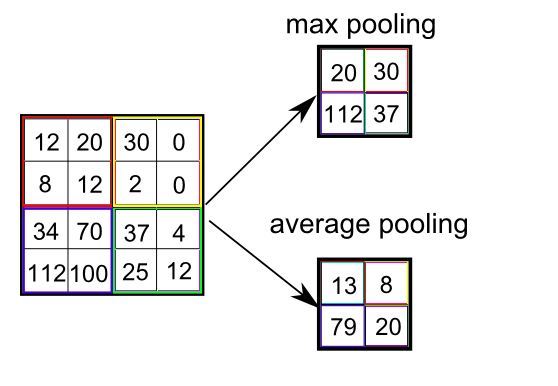
\includegraphics[width=1\linewidth]{mp}
		\end{minipage}
	\end{center}
\end{figure}

\end{frame}

\begin{frame}
	\frametitle{Объединяющий слой (pooling layer)}
		\begin{itemize}
			\item вход $W_{1} \times H_{1} \times D_{1}$
			\item 2 гиперпараметра: 
				\begin{itemize}
					\item $F$ -- ширина квадратного фильтра
					\item $S$ -- шаг фильтра
				\end{itemize}
			\item Выход $W_{2} \times H_{2} \times D_{2}$:
				\begin{itemize}
					\item $W_{2} = (W_{1} - F)/S + 1$
					\item $H_{2} = (H_{1} - F)/S + 1$
					\item $D_{2} = D_{1}$
				\end{itemize}
			\item не принято дополнять входной объект нулями
			\item чаще всего $F=3$,$S=2$ или $S=2$,$F=2$
		\end{itemize}
		\begin{figure}[h]
	\begin{center}
		\begin{minipage}[h]{0.92\linewidth}
			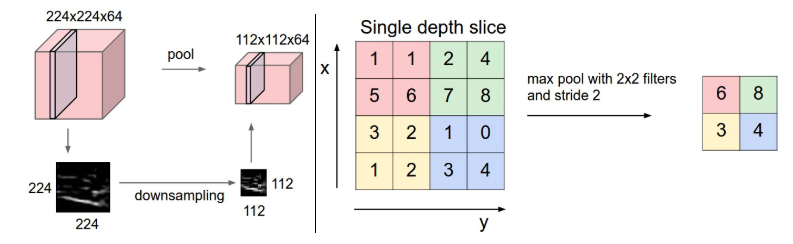
\includegraphics[width=1\linewidth]{p}
		\end{minipage}
	\end{center}
\end{figure}
\end{frame}

\begin{frame}
	\frametitle{Полносвязный слой}
	Последний из типов слоев это слой обычного многослойного персептрона. Цель слоя – классификация, моделирует сложную нелинейную функцию, оптимизируя которую, улучшается качество распознавания. Вычисление значений нейрона можно описать формулой:
	\begin{center}
		$\mathsf{x}_{\mathsf{j}}^{\mathsf{l}} = \sigma(\sum \limits_{\mathsf{i}} \mathsf{x}_{\mathsf{i}}^{\mathsf{l-1}} * \mathsf{w}_{\mathsf{i,j}}^{\mathsf{l-1}}+\mathsf{b}_{\mathsf{j}}^{\mathsf{l-1}})$,
	\end{center}
	где
	\begin{itemize}
		\item $\mathsf{x}_{j}^{l}$ -- карта признаков $\mathsf{j}$ (выход слоя $\mathsf{l}$), 
		\item $\sigma()$ -- функция активации,
		\item $\mathsf{b}^{\mathsf{l}}$ -- коэффициент сдвига слоя $\mathsf{l}$,
		\item $\mathsf{w}_{\mathsf{i,j}}^{\mathsf{l}}$ -- матрица весовых коэффициентов слоя $\mathsf{l}$.
	\end{itemize}
\end{frame}

\begin{frame}
	\frametitle{Функция активации}
	 Выделяются следующие функции активации:
		\begin{itemize}
			\item сигмойда: $\sigma(z) = \frac{1}{1 - e^{-az}}$, $a \in \mathbb{R}$;
			\item гиперболический тангенс: $\sigma(z) = \frac{e^{az} - e^{-az}}{e^{az} + e^{-az}}$;
			\item softmax: $\sigma(z)_{\mathsf{i}} = \frac{e^{z_{\mathsf{i}}}}{\sum \limits_{k=1}^{K} e^{z_{k}} }$.
		\end{itemize}
	
\end{frame}

	% \begin{frame}
 % 		\frametitle{Forward propagation}
 % 				Для выполнения операции свертки ядро ​​переворачивается на 180 градусов и скользил по входной карте, вычисляя произведение между элементом ядра и элементом карты входных данных, которое оно перекрывает,суммируя результаты для получения выходных данных в этом текущем местоположении.
	% 		\begin{figure}[h]
	% 			\begin{center}
	% 				\begin{minipage}[h]{0.42\linewidth}
	% 					\includegraphics[width=1\linewidth]{fp}
	% 				\end{minipage}
	% 			\end{center}
	% 		\end{figure}
 % 	\end{frame}
 % 	\begin{frame}
 % 		\frametitle{Forward propagation}

 % 	\end{frame}


 	% \begin{frame}
 	% 	\frametitle{Обучение CNN. Back propagation}
 	% 	Обучение полносвязных слоев.

 	% 	Ошибка формируется на последнем слое нейронов СНС и определяется как разность между выходной реакцией сети $y$ и эталоном $t$ : $\gamma_{\mathsf{j}} = \mathsf{y}_{\mathsf{j}} - t_{\mathsf{j}}$.

 	% 	Далее происходит изменение значений весов и порогов:

 	% 	\begin{center}
 	% 		$\omega_{\mathsf{ij}}(t+1) = \omega_{\mathsf{ij}}(t) - \gamma_{\mathsf{j}} F^{'}(S_{\mathsf{j}})y_{\mathsf{i}}$
 	% 	\end{center}
 		

 	% 	Ошибка для скрытого слоя с индексом  $i$ вычисляется через ошибки следующего за ним слоя с индексом $\mathsf{j}$:
 	% 	\begin{center}
 	% 		$\gamma_{\mathsf{i}} = \sum \limits_{\mathsf{j}} \mathsf{y}_{\mathsf{j}}F^{'}(S_{\mathsf{j}})\omega_{\mathsf{ji}}$.
 	% 	\end{center}

% 		Для выполнения операции свертки ядро ​​переворачивается на 180 градусов и скользил по входной карте, вычисляя произведение между элементом ядра и элементом карты входных данных, которое оно перекрывает,суммируя результаты для получения выходных данных в этом текущем местоположении.
% 			\begin{figure}[h]
% 	\begin{center}
% 		\begin{minipage}[h]{0.42\linewidth}
% 			\includegraphics[width=1\linewidth]{fp}
% 		\end{minipage}
% 	\end{center}
% \end{figure}
 	% \end{frame}

 % 	\begin{frame}
 % 		\frametitle{Обучение CNN. Back propagation}
 % 		Обучение сверточного и подвыборочного слоев.

 % 		Обратное распространение ошибки по подвыборочному слою зависит от функции пулинга. Если функция пулинга - среднее, то ошибка равномерно распространяется на $m*n$ нейронам блока предыдущего слоя. Если функция - минимум, то ошибка присваивается тому нейрону блока, с которого было взято максимальное значение по блоку. При передаче матрицы ошибок от слоя пулинга к сверточному слою служит операция обратной свертки.

 		
 % 		\begin{figure}[h]
 % 			\begin{center}
	% 	\begin{minipage}[h]{0.8\linewidth}
	% 		\includegraphics[width=1\linewidth]{180}
	% 	\end{minipage}
	% \end{center}
	% 	\end{figure}
 % 	\end{frame}

 % 	\begin{frame}
 % 		\frametitle{Обучение CNN. Back propagation}
 % 			При выполнении обратной свертки на выходе получается матрица большего размера, чем входная. Затем производится свертка входа сверточного слоя с матрицей ошибок данного слоя, повернутой на 180 градусов.
 % 			\begin{figure}[h]
 % 			\begin{center}
	% 	\begin{minipage}[h]{0.5\linewidth}
	% 		\includegraphics[width=1\linewidth]{182}
	% 	\end{minipage}
	% \end{center}
	% 	\end{figure}
	% 	Затем полученная матрица вычитается из ядра свертки данного слоя и таким образом производится изменение весов в ядре свертки сверточного слоя СНС.
 % 	\end{frame}

	% \begin{frame}
	% 	\frametitle{Backpropagation}
	% 	Алгоритм распространения ошибки сводится к следующим этапам:
	% 	\begin{itemize}
	% 		\item прямое распространение сигнала по сети, вычисления состояния нейронов;
	% 		\item вычисление значения ошибки δ для выходного слоя;
	% 		\item обратное распространение: последовательно от конца к началу для всех скрытых слоев вычисляем $\delta$ 
	% 		\item обновление весов сети на вычисленную ранее $\sigma$ ошибки.
	% 	\end{itemize}
	% 	$\mathsf{y}_{\mathsf{pj}} = \mathsf{f}_{\mathsf{j}}(\mathsf{s_{\mathsf{pj}}})$, где $\mathsf{y}_{\mathsf{pj}}$ -- активированное состояние нейрона, $\mathsf{f}_{\mathsf{j}}$ -- функция активации, $s_{\mathsf{pj}} = \sum \limits_{i} \mathsf{w}_{\mathsf{ij}} \mathsf{y}_{\mathsf{pi}}$ - взвешенная сумма выходов связанных нейронов предыдущего слоя на вес связи.

	% \end{frame}
	\begin{frame}
\frametitle{Forwardpropagation and Backpropagation}
По сути, к снс применим обычный алгоритм прямого и обратного распространения, так как она подходит по определение обычной нс, мы просто обнуляем большинство весов, которые скорее всего не дают вклада.\\
\vspace{0.3cm}
Но за счет специфичного построения последующих слоев, у нас появляется возможность переписать эти алгоритмы в более удобную для вычислений форму.\\
\vspace{0.3cm}
Далее представлен алгоритм, по которому усовершенствуются Forwardpropagation и Backpropagation.
\end{frame}

	\begin{frame}
		\frametitle{Forwardpropagation}
		Операция свертки может быть записана так, как описано на рисунке ниже.
		\begin{figure}[h]
			\begin{center}
				\begin{minipage}[h]{0.92\linewidth}
					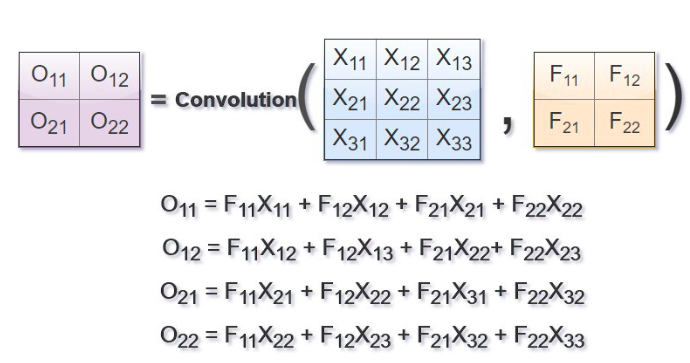
\includegraphics[width=1\linewidth]{fv}
				\end{minipage}
			\end{center}
		\end{figure}

	\end{frame}

	\begin{frame}
		\frametitle{Forwardpropagation}
		Теперь, чтобы вычислить градиенты фильтра $F$ относительно ошибки $E$, необходимо решить уравнения, которые можно записать в форме операции свертки.

		\begin{figure}[h]
			\begin{center}
				\begin{minipage}[h]{0.92\linewidth}
					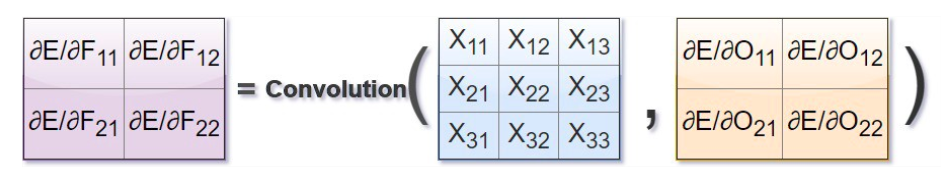
\includegraphics[width=1\linewidth]{fv1}
				\end{minipage}
			\end{center}
		\end{figure}
	\end{frame}

\begin{frame}
	\frametitle{Forwardpropagation}
	Точно так же мы можем найти градиенты входной матрицы $X$ относительно ошибки $E$.
\begin{figure}[h]
			\begin{center}
				\begin{minipage}[h]{0.52\linewidth}
					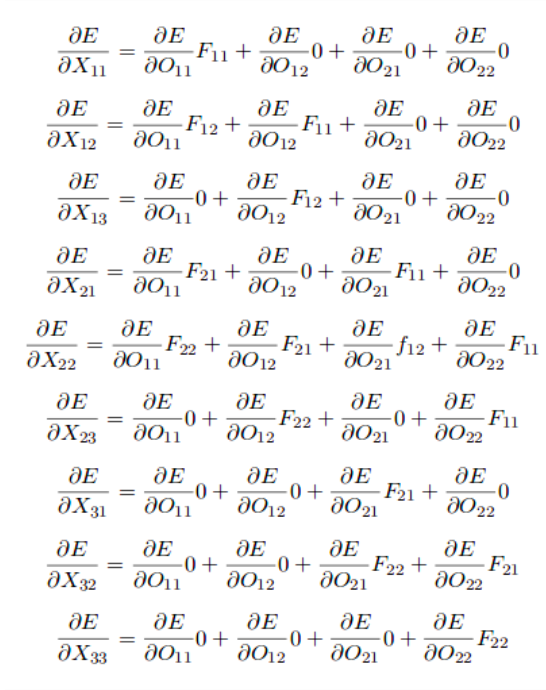
\includegraphics[width=1\linewidth]{fv2}
				\end{minipage}
			\end{center}
		\end{figure}

\end{frame}

\begin{frame}
	\frametitle{Backpropagation}
	Теперь вышеприведенные вычисления могут быть получены с помощью операции свертки другого типа, известной как полная свертка. Чтобы получить градиенты входной матрицы, необходимо повернуть фильтр на $180$ градусов и рассчитать полную свертку повернутого фильтра по градиентам выходного сигнала относительно ошибки.
	\begin{figure}
		\begin{center}
				\begin{minipage}[h]{1.1\linewidth}
					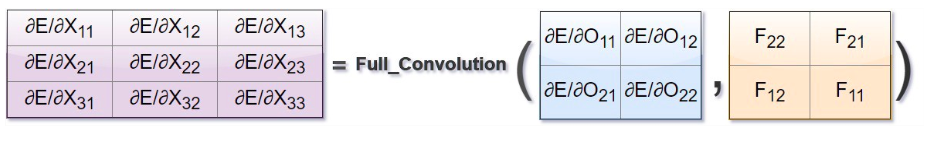
\includegraphics[width=1\linewidth]{bv1}
				\end{minipage}
			\end{center}
		\end{figure}
\end{frame}

\begin{frame}
	\frametitle{Backpropagation}
	Полная свертка может быть визуализирована как выполнение процедуры, представленной на рисунке ниже.
	\begin{figure}
		\begin{center}
				\begin{minipage}[h]{0.65\linewidth}
					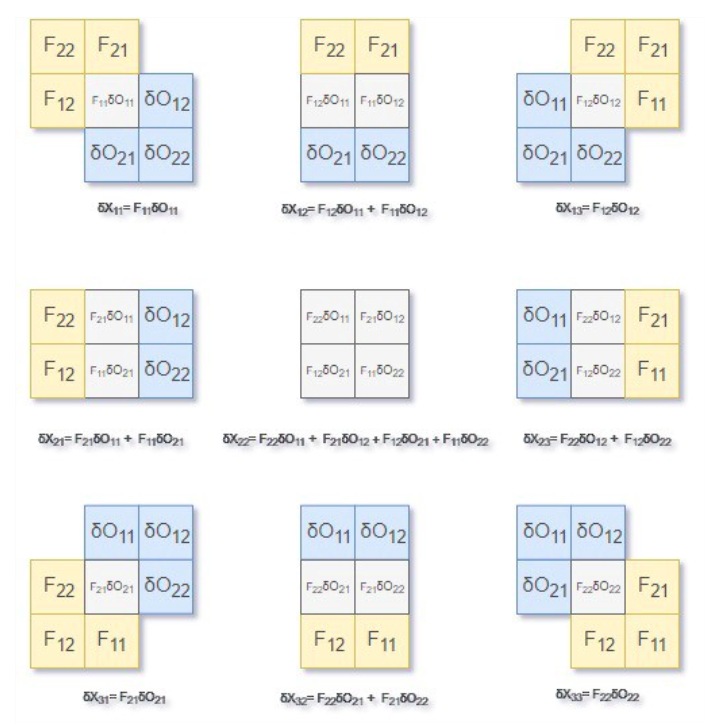
\includegraphics[width=1\linewidth]{bv2}
				\end{minipage}
			\end{center}
		\end{figure}
\end{frame}

\end{document}
